\chapter{Teoria}
\label{c3}

\section{Wstęp}
\label{c31}

W niniejszym rozdziale zawarto opis architektury oraz główne komponenty wykorzystywane przez App Inventora. Pomoże to zrozumieć zalety oraz wady powyższego narzędzia.

\section{App Inventor}
\label{c21}

App Inventor jest systemem pozwalającym na tworzenie aplikacji poprzez używanie jedynie przeglądarki internetowej. Jest to zatem aplikacja internetowa umożliwiająca zredagowanie programu informatycznego nawet przez użytkowników dysponujących niewielkim zasobem profesjonalnej  wiedzy i umiejętności z zakresu programowania.  

\subsection{Historia}

Aplikacja została uruchomiona w lipcu 2010 roku. Można było wtedy skorzystać z niej, kiedy programista złożył odpowiednie żądanie. W grudniu platforma została udostępniona publicznie. W drugiej połowie 2011 roku Google udostępnił kod źródłowy oraz został sponsorem wykładając fundusze na  stworzenie Centrum Nauki o Urządzeniach Mobilnych MIT (\english{MIT Center for Mobile Learning}). Wersja MIT została uruchomiona w marcu 2012 roku.\cite{android:39}

W grudniu 2013 została wydana druga wersja systemu App Inventor. Starszą wersję określono jako Classic. Oba narzędzia są do siebie bardzo podobne, jednak projektów stworzonych w pierwszej wersji systemu nie można zaimportować do wersji nowszej. W niniejszej pracy magisterskiej skupiono się na nowszej wersji App Inventora. 

Potencjał aplikacji jest bardzo duży. Można to stwierdzić obserwując ilość aktywnych użytkowników. W maju 2014 ich liczba wynosiła 87tys. tygodniowo. Liczba zarejestrowanych użytkowników to 1,9mln w 195 krajach świata. Stworzyli oni łącznie 4,7mln projektów.\cite{article:appinventor1}

\subsection{Architektura}
\label{c32}

Każda aplikacja ma swoją wewnętrzną strukturę, którą trzeba dokładnie zrozumieć, aby tworzyć efektywne oprogramowanie. Architektura aplikacji składa się głównie z 2 części: komponenty oraz ich zachowanie. Można z pewnym dystansem przyjąć, że za komponenty odpowiada widok Designera, a za zachowanie komponentów widok edytora.

\begin{figure}[th] 
\centering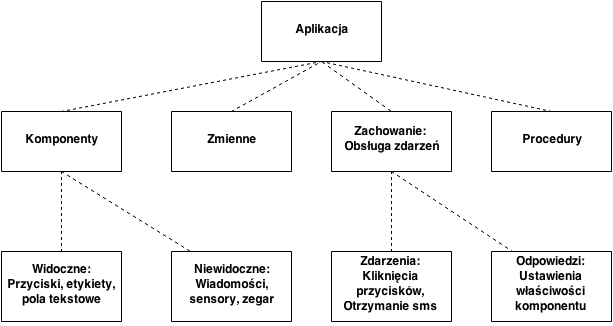
\includegraphics[width=12cm]{figures/architektura}
\caption{Architektura aplikacji stworzonej przez App Inventora\cite{appinventor:architektura}}
\end{figure}

\subsection{Komponenty}
\label{c321}

Komponenty można podzielić na 2 rodzaje: widoczne oraz niewidoczne. 
\begin{itemize}
\item Widoczne użytkownik widzi gołym okiem. Należą do nich przyciski, etykiety, pola tekstowe. Definiują one interfejs użytkownika.
\item Niewidocznych komponentów, jak sama nazwa wskazuje, użytkownik nie widzi. Nie są one częścią interfejsu. Dostarczają one dostępu do wbudowanych funkcjonalności telefonu. Są to różne sensory np. akcelerometr, moduł gps, komponent zamiany tekstu na mowę itp.
\end{itemize}

Oba rodzaje komponentów posiadają zbiór swoich właściwości. Właściwości danego komponentu są to informacje jakie komponent posiada. Etykieta posiada między innymi rodzaj, wielkość, dekorację, kolor czcionki, wielkość, widoczność etykiety. Użytkownik nie widzi danych właściwości, obserwuje on rezultat konkretnych ustawień na ekranie urządzenia.

\subsection{Zachowanie aplikacji}
\label{c322}
Zrozumienie zasady tworzenia komponentów i ich właściwości jest proste. Nazwy komponentów są intuicyjne, więc nie powinno być problemu z odnalezieniem tego, który interesuje programistę. Z drugiej strony zachowanie komponentów może okazać się bardziej skomplikowane. Mimo wszystko App Inventor stara się wizualizować bloki opisujące zachowanie w jak najprostszej formie.

Kiedy zaczynano pisać aplikacje, można było je porównać do recept, gdzie ciąg zdarzeń ukazany jest jako liniowa sekwencja instrukcji. Typowa aplikacja może uruchomić transakcję w banku, dokonać pewnych obliczeń, zmodyfikować stan konta i na koniec wyświetlić nowe saldo.\cite{appinventor:architektura}

W dzisiejszych czasach większość aplikacji nie wpasowuje się w powyższy schemat. Zamiast wykonywać ciąg instrukcji w odpowiedniej kolejności, reagują na zdarzenia, które są inicjowane przez użytkownika danej aplikacji. Jednym z przykładów jest kliknięcie przycisku lub trzęsienie telefonem, który jest zaprogramowany tak, aby na każdy bodziec móc umieć odpowiedzieć. Wiele zdarzeń jest inicjowanych przez użytkownika, ale są też wyjątki. Aplikacja może reagować na zdarzenia, które w nie wymagają interakcji z użytkownikiem. Często są to niewidoczne komponenty umieszczone w Designerze. Poniższy rysunek prezentuje aplikację otoczoną wieloma zdarzeniami.

\begin{figure}[th] 
\centering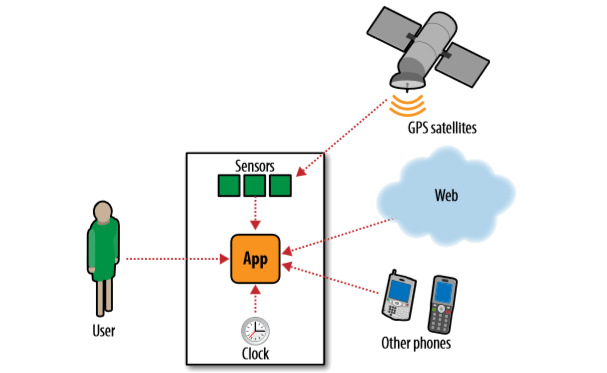
\includegraphics[width=10cm]{figures/events}
\caption{Aplikacja reagująca na zdarzenia zewnętrzne i wewnętrzne\cite{appinventor:architektura}}
\end{figure}

Jednym z powodów dlaczego App Inventor jest tak intuicyjny jest zastosowanie prostej koncepcji nazywania zdarzeń. Zdefiniowanie zdarzenia polega na przeciągnięciu go z palety na główny ekran, a następnie napisanie konkretnego zachowania. Przykładem takiego zdarzenia jest obsługa akcelerometru. Po zatrzęsieniu telefonem, pojawia się tekst \emph{Shaking!}.

\begin{figure}[th] 
\centering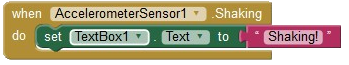
\includegraphics[width=10cm]{figures/shakingEvent}
\caption{Obsługa zdarzenia trzęsienia telefonem}
\end{figure}

Zdarzenia można podzielić w zależności od jego typu:
\begin{itemize}
\item Zainicjowane przez użytkownika - najbardziej popularny typ zdarzenia - głównie jest to obsługa zdarzeń dotyku ekranu.
\item Inicjalizujące - są wykonywane, gdy dany komponent jest tworzony.
\item Czasowe - są uruchamiane, co pewien interwał czasowy.
\item Animacje - są zależne od obiektów (spritów) które zostały stworzone. Mogą zostać uruchomione gdy obiekty ze sobą kolidują, wylatują poza ekran.
\item Zewnętrzne - są uruchamiane gdy urządzenie odbierze jakiś sygnał zewnętrzny typu, odczyt pozycji urządzenia z satelity, reakcja na przychodzący sms.
\end{itemize}

Programowanie aplikacji odbywa się poprzez zdefiniowanie interfejsu, a następnie napisanie zachowania danej aplikacji, dla różnych zdarzeń, które mogą wystąpić. Inaczej mówiąc, komponenty tworzone są najpierw w Designerze i tam przypisywane są do nich właściwości. Programista po otrzymaniu interesującego go wyglądu może przystąpić do opisu zdarzeń.

\subsection{Debugowanie aplikacji}
\label{c33}

Najłatwiejszy sposób instalacji i testowania aplikacji odbywa się przez wifi. Musimy pobrać dodatkową aplikację na urządzenie z systemem Android. Następnie na stronie App Inventora uruchamiamy opcję połączenia z telefonem i pojawia nam się na monitorze kod QR, który skanujemy telefonem, z pomocą ściągniętej aplikacji.Po wykonaniu powyższych czynności następuje automatyczna instalacja aplikacji na telefonie. Dzięki aplikacji następuje również automatyczne uaktualnienie wprowadzonych zmian, nie zachodzi konieczność jej ponownego uruchamiania. 
Powyżej opisany sposób debugowania aplikacji jest rekomendowany, ale należy wspomnieć o istnieniu dwóch innych możliwości. Jedna z nich odnosi się do przypadku, gdy nie posiadamy urządzenia z systemem Android. Możemy wówczas użyć emulatora. Trzecia opcja to możliwość połączenia telefonu z komputerem i aplikacją przez kabel USB. 

\section{Praca ze środowiskiem App Inventor}

\subsection{Podłączenie telefonu/tabletu}

Aby zacząć pracę z App Inventorem należy połączyć telefon z platformą. Designer i Block Editor działają całkowicie w przeglądarce. Aby zobaczyć aplikację podczas budowania trzeba wybrać jedną z trzech możliwości.\cite{android:40}

Pierwszą opcją jest rekomendowaną przez App Inventora jest użycie WiFi. Nie trzeba wtedy instalować żadnych programów na komputerze. Jedną aplikacją, którą należy zainstalować jest \emph{App Inventor Companion App}.

\begin{figure}[H] 
\centering
\includegraphics[width=8cm]{figures/option1wifi}
\caption{Połączenie telefonu przez WiFi}
\end{figure}

Kolejną opcja jest dla osób nie posiadających urządzenia z systemem Android. Należy zainstalować oprogramowanie umożliwiające uruchomienie emulatora. Jest to również przydatna opcja, gdy nauczyciel musi pracować z grupą studentów i musi każdemu z nich zapewnić urządzenie z Androidem.\cite{android:40}

\begin{figure}[H] 
\centering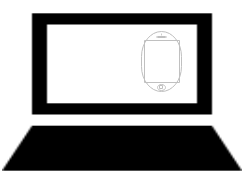
\includegraphics[width=6cm]{figures/option2emulator}
\caption{Korzystanie z emulatora zainstalowanego na komputerze}
\end{figure}

Ostatnią opcją jest zainstalowanie odpowiedniego oprogramowania, aby połączyć zewnętrzne urządzenie z systemem Android za pomocą USB. Może to być przydane również gdy niektóre zapory sieciowe w szkołach i innych organizacjach blokują dosęp do WiFi.\cite{android:40}

\begin{figure}[H] 
\centering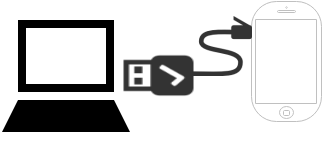
\includegraphics[width=6cm]{figures/option3usb}
\caption{Korzystanie z telefonu podłączonego za pomocą USB}
\end{figure}

\subsection{Współdzielenie i budowanie aplikacji}

Istnieje możliwość współdzielenia stworzonych aplikacji w wykonywalnym formacie \emph{.apk}, które mogą zostać zainstalowane na urządzeniu lub w wersji dającej możliwość edycji w platformie - jest to format \emph{.aia}. Dodatkowo aplikacje stowrzone za pomocą App Inventora można udostępniać w markecie Google Play.\cite{android:41}

\subsection{Porady i wskazówki}

Istnieje kilka elementów, które ułatwiają pracę z tworzonymi aplikacjami. Poniżej zostały one wskazane.\cite{android:42}

\begin{itemize}
\item Tworzenie komentarzy - platforma daje możliwość pisania komentarzy przy zdefiniowanych blokach. Mimo że jest to programowanie wizualne, warto to robić, aby inni, którzy będą patrzeć na stworzoną aplikację szybciej zrozumieli jej działanie.
\item Kondensowanie bloków - tworząc większy projekt, ilość bloków na ekranie osiąga znaczącą liczbę i nie jest łatwo programiście się odnaleźć. App Inventor daje możliwość ukrywania bloków, aby zrobić więcej miejsca na ekranie i tym samym ułatwiając tworzenie aplikacji.
\item Szybkie wybieranie - po stworzeniu kilku aplikacji programista ma świadomość jakie bloki oferuje App Inventor. Aby w szybki sposób stowrzyć kolejne wystarczy, że zacznie on pisać potrzebną mu nazwę bloku. Dana czynność wyświetli listę, pasujących do wpisanego słowa, bloków.
\item Szybkie usuwanie - zamiast przeciągania bloków do ikony śmietnika, można użyć klawisza \emph{DEL}.
\item Kopiuj/Wklej - jeżeli istnieje potrzeba wykorzystania jeszcze raz wcześniej stworzonych już bloków, App Inventor umożliwia ich skopiowanie i wklejenie.
\end{itemize}

\subsection{Nowości w 2 wersji}

App Inventor różni się od poprzedniej wersji w wielu aspektach.\cite{android:43} Niektóre elementy wydają się tak naturalne, że niektórzy mogą się zastanawiać, jak programiści mogli używać App Inventora w poprzedniej wersji. Poniżej zaprezentowo kilka z nich:

\begin{itemize}
\item Listy rozwijane - niektóre bloki w App Inventorze mają do wyboru listę rozwijaną odpowiadającą za właściwości komponentu.\cite{android:44} 
\begin{figure}[H] 
\centering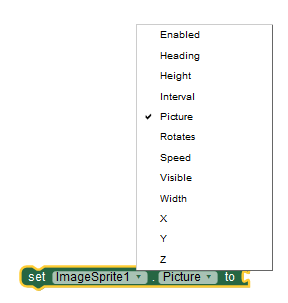
\includegraphics[width=6cm]{figures/dropdowns}
\caption{Wykorzystanie zmiany właściwości za pomocą listy rozwijanej}
\end{figure}

\item Mutatory - nowa funkcja dająca możliwość niektórym blokom rozbudowania się lub pomniejszenia, a nawet zmianę dotychczasowego zachowania. Mutatory mogą zmieniać kształt. Programista ma możliwość przeciągnięcia dodatkowych mniejszych bloczków i przypisanie ich do bloku głównego.\cite{android:45} Poniżej na obrazku zaprezentowane są często używane mutatory:

\begin{figure}[H] 
\centering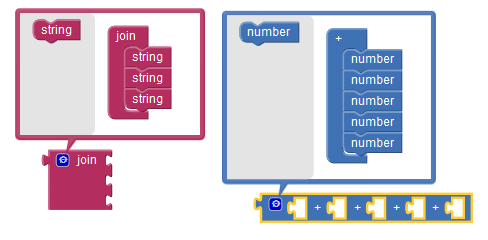
\includegraphics[width=10cm]{figures/mutators}
\caption{Mutator łączenia tekstu oraz działań matematycznych}
\end{figure}

\item Zmienne lokalne i globalne - zmienna globalna jest komponentem dostępnym w każdym bloku. Programista może w każdym miejscu zmienić lub odczytać jej wartość. Zmienne lokalne deklarowane są wewnątrz funkcji lub jest to argument przekazany do funkcji. Oznaczna to że można uzyskać do nich dostęp tylko w zadeklarowanym obszarze.\cite{android:46}

\item Emulator - ze względu braku urządzenia z systemem Android istnieje możliwość tworzenia aplikacji używając emulatora. Działa on tak samo jak urządzenie zewnętrzne, tylko że wyświetla się na monitorze komputera. Większość szkół nie posiada funduszy na dużą liczbę urządzeń z systemem Android. Uczniowe tworzą wtedy aplikacje za pomocą emulatora, a następnie używają urządznia do końcowych testów.\cite{android:47}

\item Kolory - w drugiej wersji App Inventor dostarczył bloki dające możliwość wybrania koloru. Programista może wybrać kolor z predefiniowanej palety, lub skorzystać z odpowiedniego bloku podając wartości RGB.\cite{android:48}

\item App Inventor działa całkowicie w przeglądarcie internetowej. Poprzednio należało zainstalować plik Javy nazwany Block Editor. Aktualnie Block Editor jest to inny tryb, w który można się przełączyć z przeglądarce.\cite{android:43}

\item Wyeksportowany kod posiada rozszerzenie \emph{.aia} zamiast \emph{.zip} \cite{android:43}

\end{itemize}

\section{Główne komponenty}
\label{c22}

App Inventor celowo ułatwia programowanie poprzez wizualizację tworzonych komponentów i intuicyjny interfejs. App Inventor składa się z 3 głównych komponentów, jakimi są:
\begin{itemize}
\item App Inventor Designer
\item App Inventor Blocks Editor
\item Android Device Emulator
\end{itemize}

\subsection{App Inventor Designer}
\label{c221}

Jednym z głównych widoków których można używać jest widok Designera. Projektowanie interfejsu użytkownika polega na przeciąganiu komponentów z dostępnej palety, wliczając w to także niewidoczne komponenty, takie jak sensory. W tym widoku można również zmieniać właściwości obiektów, które zostały stworzone. Między innymi istnieje możliwość zmiany położenia, wielkości, układu (pionowy, poziomy).

Designer jest zaprojektowany jako zwykła aplikacja internetowa. Tak więc uruchamia się go, jak zwykłą stronę internetową wpisując jej adres www.

\begin{figure}[th] 
\centering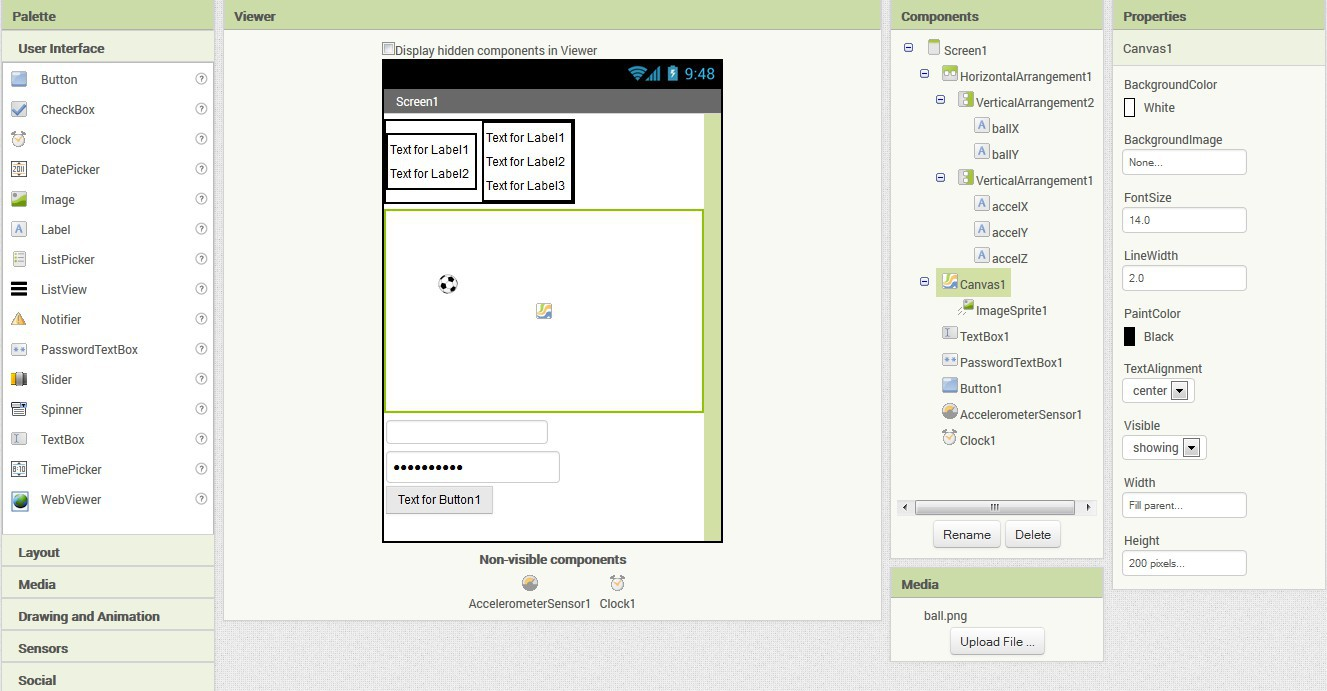
\includegraphics[width=10cm]{figures/designer}
\caption{App Inventor Designer}
\end{figure}

\subsection{App Inventor Blocks Editor}
\label{c222}

Drugim widokiem jest Blocks Editor. Zachowanie aplikacji zostaje tutaj zaprogramowane poprzez połączenie odpowiednich bloków. Istnieje możliwość korzystania z bardziej generalnych komponentów, a także z bardziej specyficznych. Dla każdego komponentu, który został stworzony w interfejsie graficznym (Designerze) są dostępne bloki mówiące, co tak naprawdę jest możliwe do zrobienia. Wygląda to w ten sposób, że komponenty są przciągane z dostępnej palety metodą "przeciągnij i upuść", a następnie łączone jak puzzle.

Ta część aplikacji normalnie reprezentowana jest przez kod napisany przez programistę. Zatem napisanie zachowania aplikacji odbywa się poprzez łączenie puzzli, bez wymogu znajomości języka Java.

\begin{figure}[H] 
\centering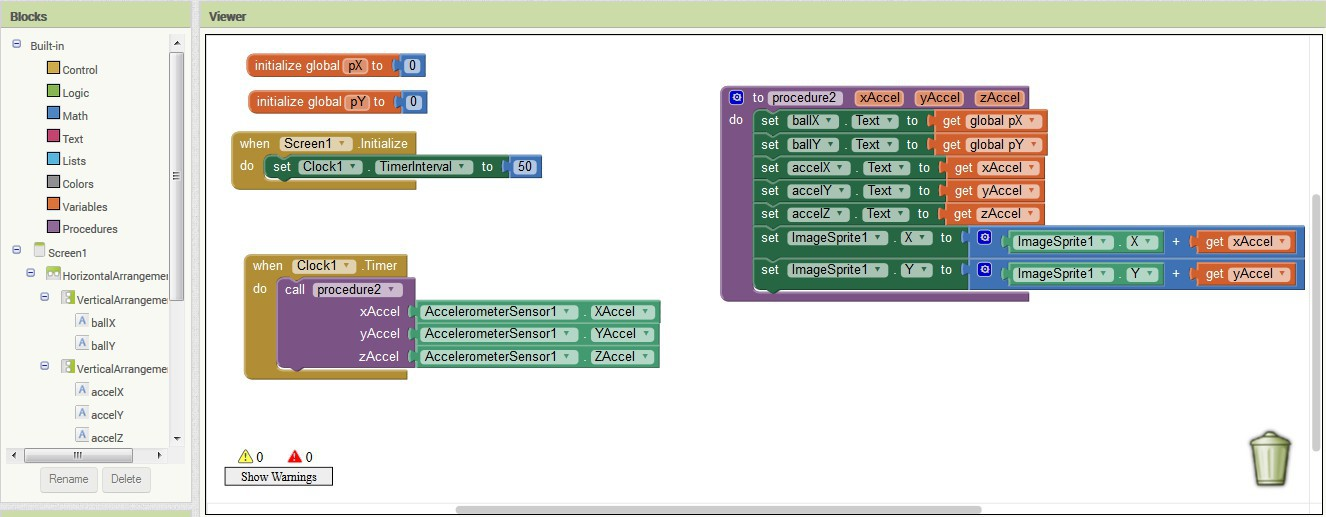
\includegraphics[width=10cm]{figures/editor}
\caption{App Inventor Blocks Editor}
\end{figure}

\subsection{Android Device Emulator}
\label{c223}

Android Device Emulator jest to emulator telefonu lub tabletu. Przedstawia on wirtualną wersję smartphonu, w której znajdują się obsługa dotyku ekranu, przyciski systemowe oraz typowe funkcje.

Wprowadzone zmiany, natychmiast reflektują na działanie aplikacji. Nie ma potrzeby jakiejkolwiek kompilacji i uruchamiania aplikacji od nowa. Jeżeli aplikacja zostanie uruchomiana, kompilacja zmienionych fragmentów oraz zainstalowanie ich na emulatorze dzieje się w czasie rzeczywistym. Jest to bardzo wygodna opcja budowania aplikacji i testowania jej. Zmiany, które zrobimy, są od razu widoczne na ekranie.

\begin{figure}[H] 
\centering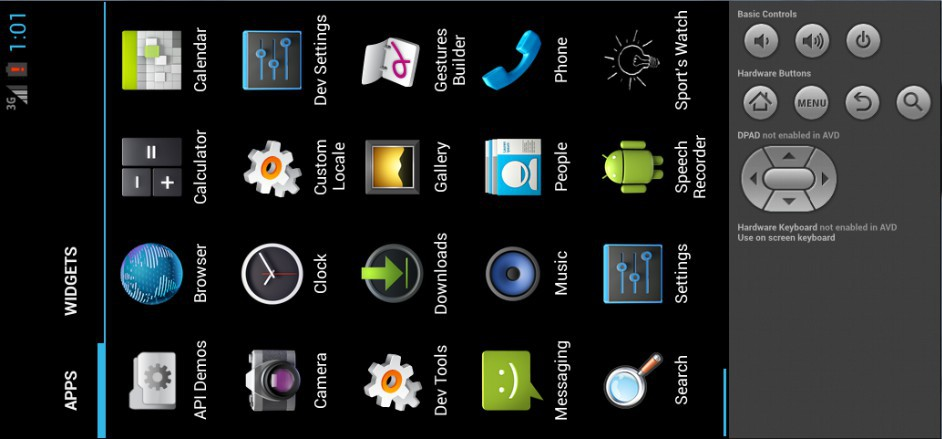
\includegraphics[width=10cm]{figures/emulator}
\caption{Android Device Emulator}
\end{figure}



